\section{Langkah-Langkah Percobaan}

Pada praktikum ini, kami menggunakan dua buah laptop sebagai PC1 dan PC2, dua perangkat Mikrotik sebagai router, serta tiga kabel LAN untuk membangun topologi jaringan. PC1 terhubung ke Router1 melalui ether2, PC2 terhubung ke Router2 melalui ether2, dan koneksi antar router dilakukan melalui ether1 masing-masing. Untuk melakukan konfigurasi, kami menggunakan perangkat lunak Winbox yang terhubung melalui MAC Address. Langkah pertama adalah mengatur alamat IPv6 pada interface ether1 di kedua router agar koneksi antar-router dapat terbentuk. Setelah itu, kami mengatur IP address pada interface ether2 masing-masing router yang terhubung ke PC.

Setelah konfigurasi selesai, kami melakukan pengujian koneksi antar-router menggunakan fitur ping di Winbox. Hasilnya menunjukkan bahwa koneksi berhasil, menandakan bahwa alamat IPv6 telah dikonfigurasi dengan benar. Selanjutnya, kami mengonfigurasi alamat IPv6 secara manual pada masing-masing laptop agar berada pada jaringan yang sesuai dengan router yang terhubung. Pengujian dilakukan kembali, kali ini antara PC1 dan PC2, untuk memastikan konektivitas antar end-device. Setelah tahap routing statis berhasil, kami melanjutkan ke konfigurasi routing dinamis menggunakan protokol OSPFv3. Kami menambahkan instance OSPFv3 di masing-masing router, kemudian menambahkan interface yang akan digunakan agar OSPF dapat bertukar informasi routing.

Pengujian konektivitas kembali dilakukan setelah konfigurasi OSPFv3 selesai. Ping antar-router dan antar-laptop menunjukkan hasil sukses, yang berarti proses routing dinamis IPv6 telah berjalan sebagaimana mestinya. Dengan demikian, seluruh rangkaian percobaan mencakup konfigurasi awal, implementasi routing statis, serta transisi dan penerapan routing dinamis berbasis protokol OSPFv3.

\section{Analisis Hasil Percobaan}

Berdasarkan hasil percobaan, kami berhasil memahami dan menerapkan konsep routing IPv6, baik secara statis maupun dinamis. Pada tahap routing statis, konfigurasi manual IP address dan penambahan rute berhasil menciptakan komunikasi antar-router dan antar-PC. Namun, proses ini cukup memakan waktu dan rawan kesalahan apabila terdapat kekeliruan pada input alamat atau gateway. Hal ini menegaskan bahwa routing statis lebih cocok digunakan pada jaringan yang kecil atau topologi yang jarang mengalami perubahan.

Sementara itu, implementasi routing dinamis menggunakan OSPFv3 menunjukkan kelebihan dari sisi efisiensi dan kemudahan manajemen jaringan. Dengan hanya mengaktifkan OSPF pada masing-masing interface, router secara otomatis dapat bertukar informasi routing dan membentuk jalur komunikasi antar jaringan. Hasil pengujian ping antar-router maupun antar-PC menunjukkan bahwa jaringan berjalan dengan baik setelah OSPFv3 dikonfigurasi. Penggunaan routing dinamis sangat bermanfaat untuk jaringan berskala menengah hingga besar yang dinamis dan membutuhkan adaptasi cepat terhadap perubahan topologi. Praktikum ini memberikan pemahaman yang konkret tentang bagaimana IPv6 dapat diimplementasikan dalam skenario nyata serta perbedaan mendasar antara metode routing statis dan dinamis.

\section{Hasil Tugas Modul}

Pada tugas ini dilakukan simulasi jaringan IPv6 menggunakan dua buah router Cisco 1941 dan dua buah laptop/PC sebagai end device, dengan topologi sebagai berikut:

\begin{center}
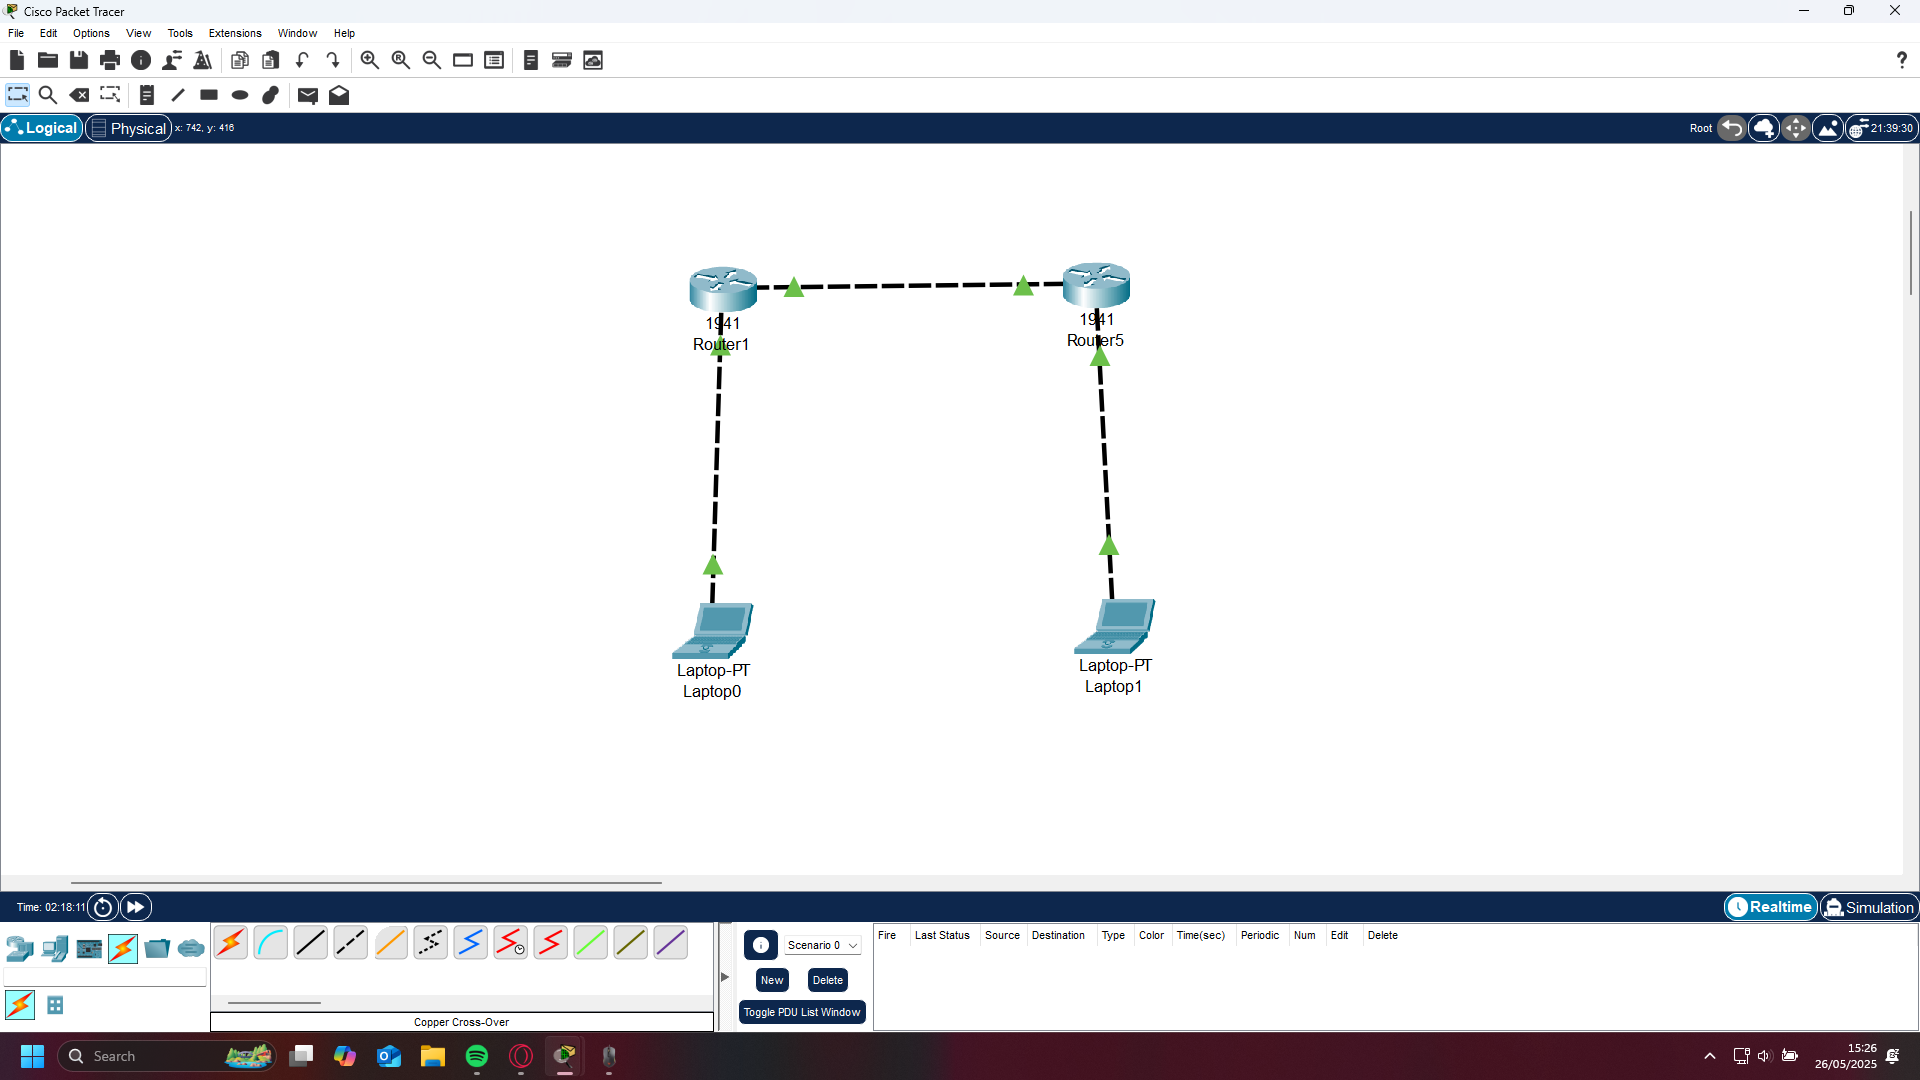
\includegraphics[width=0.8\textwidth]{P1/img/topologi_simulasi_ipv6.png}
\end{center}

\subsection*{Konfigurasi Alamat IP}

\begin{itemize}
    \item \textbf{Laptop yang terhubung ke Router 1}
    \begin{itemize}
        \item IP Address: \texttt{2001:db8:a::100/64}
        \item Gateway: \texttt{2001:db8:a::1}
        \item DNS: \texttt{2001:4860:4860::8888}
    \end{itemize}

    \item \textbf{Laptop yang terhubung ke Router 2}
    \begin{itemize}
        \item IP Address: \texttt{2001:db8:b::100/64}
        \item Gateway: \texttt{2001:db8:b::1}
        \item DNS: \texttt{2001:4860:4860::8888}
    \end{itemize}
\end{itemize}

\subsection*{Konfigurasi Router}

\begin{itemize}
    \item \textbf{Router 1 (R1)}
    \begin{itemize}
        \item Interface ke PC (Ethernet 2): \texttt{2001:db8:a::1/64}
        \item Interface antar-router: \texttt{2001:db8:1::1/64}
        \item Routing statis ke jaringan Router 2:
        \begin{verbatim}
ipv6 route 2001:db8:b::/64 2001:db8:1::2
        \end{verbatim}
    \end{itemize}

\begin{figure}[H]
    \centering
    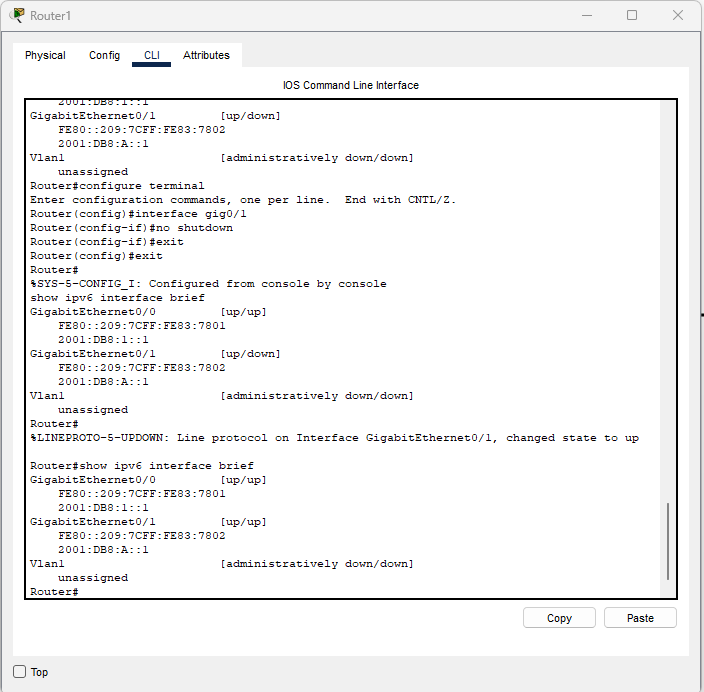
\includegraphics[width=0.48\textwidth]{P1/img/router1 konfigurasi ip.png}
    \caption{Konfigurasi IP Pada Router 1}
\end{figure}

\begin{figure}[H]
    \centering
    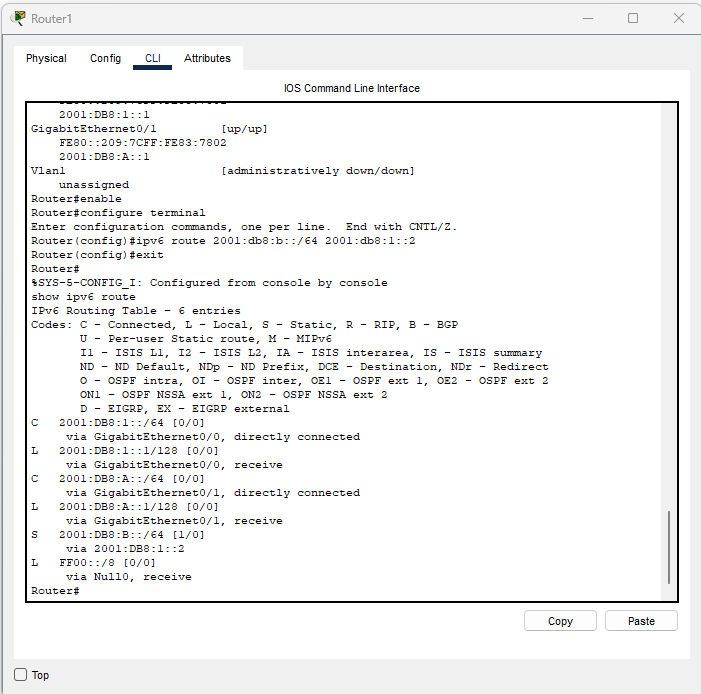
\includegraphics[width=0.48\textwidth]{P1/img/router1 route list.png}
    \caption{List Route Pada Router 1}
\end{figure}

    \item \textbf{Router 2 (R2)}
    \begin{itemize}
        \item Interface ke PC (Ethernet 2): \texttt{2001:db8:b::1/64}
        \item Interface antar-router: \texttt{2001:db8:1::2/64}
        \item Routing statis ke jaringan Router 1:
        \begin{verbatim}
ipv6 route 2001:db8:a::/64 2001:db8:1::1
        \end{verbatim}

\begin{figure}[H]
    \centering
    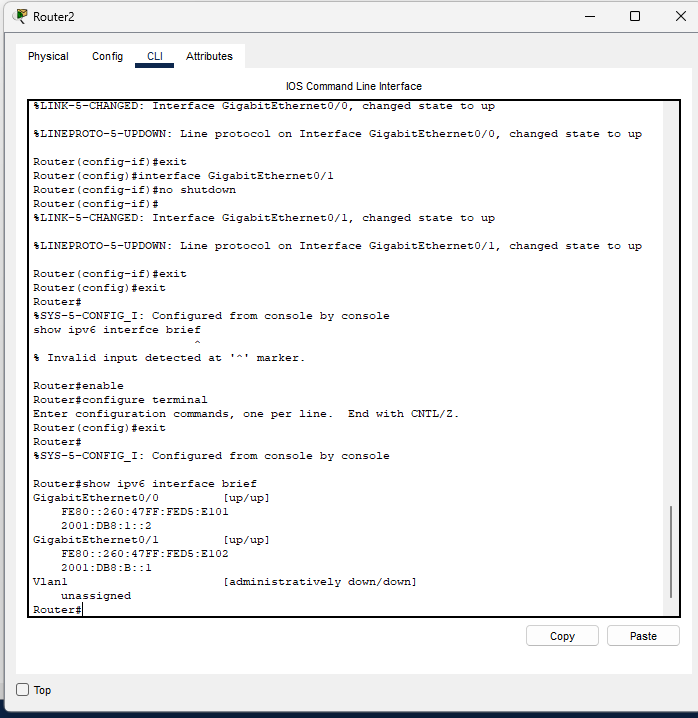
\includegraphics[width=0.48\textwidth]{P1/img/router2 konfigurasi ip.png}
    \caption{Konfigurasi IP Pada Router 2}
\end{figure}

\begin{figure}[H]
    \centering
    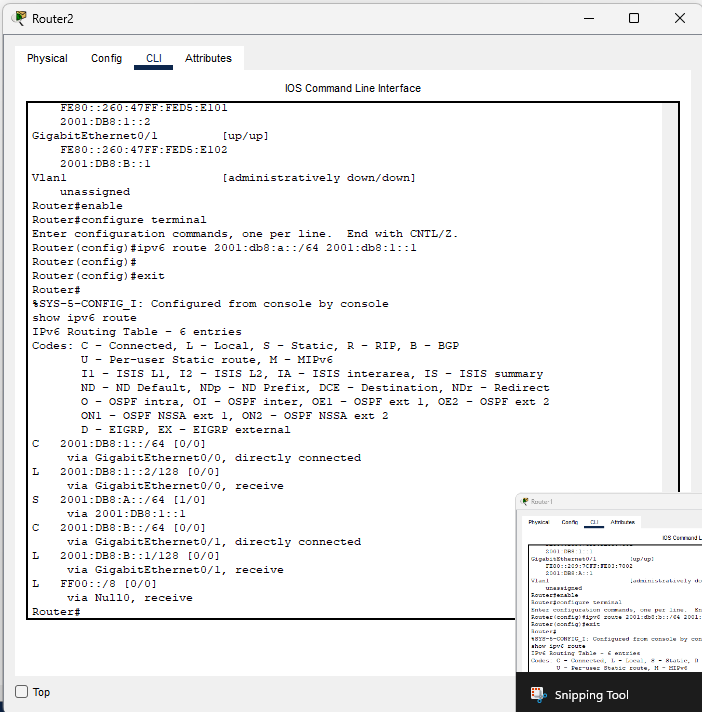
\includegraphics[width=0.48\textwidth]{P1/img/router2 route list.png}
    \caption{List Route Pada Router 2}
\end{figure}
        
    \end{itemize}
\end{itemize}

\subsection*{Pengujian Koneksi}

Pengujian konektivitas dilakukan dengan perintah \texttt{ping} dari Laptop 1 ke Laptop 2 menggunakan alamat IPv6. Hasilnya menunjukkan bahwa koneksi antar perangkat berhasil dilakukan setelah konfigurasi routing statis IPv6 diterapkan dengan benar.

\subsection*{Kesimpulan}

Dari hasil simulasi ini, dapat disimpulkan bahwa:
\begin{itemize}
    \item IPv6 dapat dikonfigurasi secara statis dengan efisien pada topologi sederhana dua router.
    \item Routing statis memungkinkan komunikasi antara dua jaringan yang berbeda melalui router yang telah dikonfigurasi dengan benar.
    \item Penetapan alamat IP, gateway, dan DNS secara manual tetap efektif dalam skenario jaringan kecil.
\end{itemize}

\section{Kesimpulan}
Melalui praktikum ini, kami mempelajari konfigurasi routing IPv6 baik secara statis maupun dinamis. Routing statis memberikan kontrol penuh atas arah lalu lintas data, namun kurang fleksibel. Sebaliknya, routing dinamis lebih efisien dalam jaringan yang bersifat dinamis atau kompleks karena dapat menyesuaikan rute secara otomatis. Praktikum ini juga memberikan pemahaman mendalam tentang pengelolaan jaringan IPv6 serta penggunaan perangkat Mikrotik dan Winbox dalam mengelola jaringan.

\section{Lampiran}
\subsection{Dokumentasi saat praktikum}
\begin{figure}[H]
    \centering
    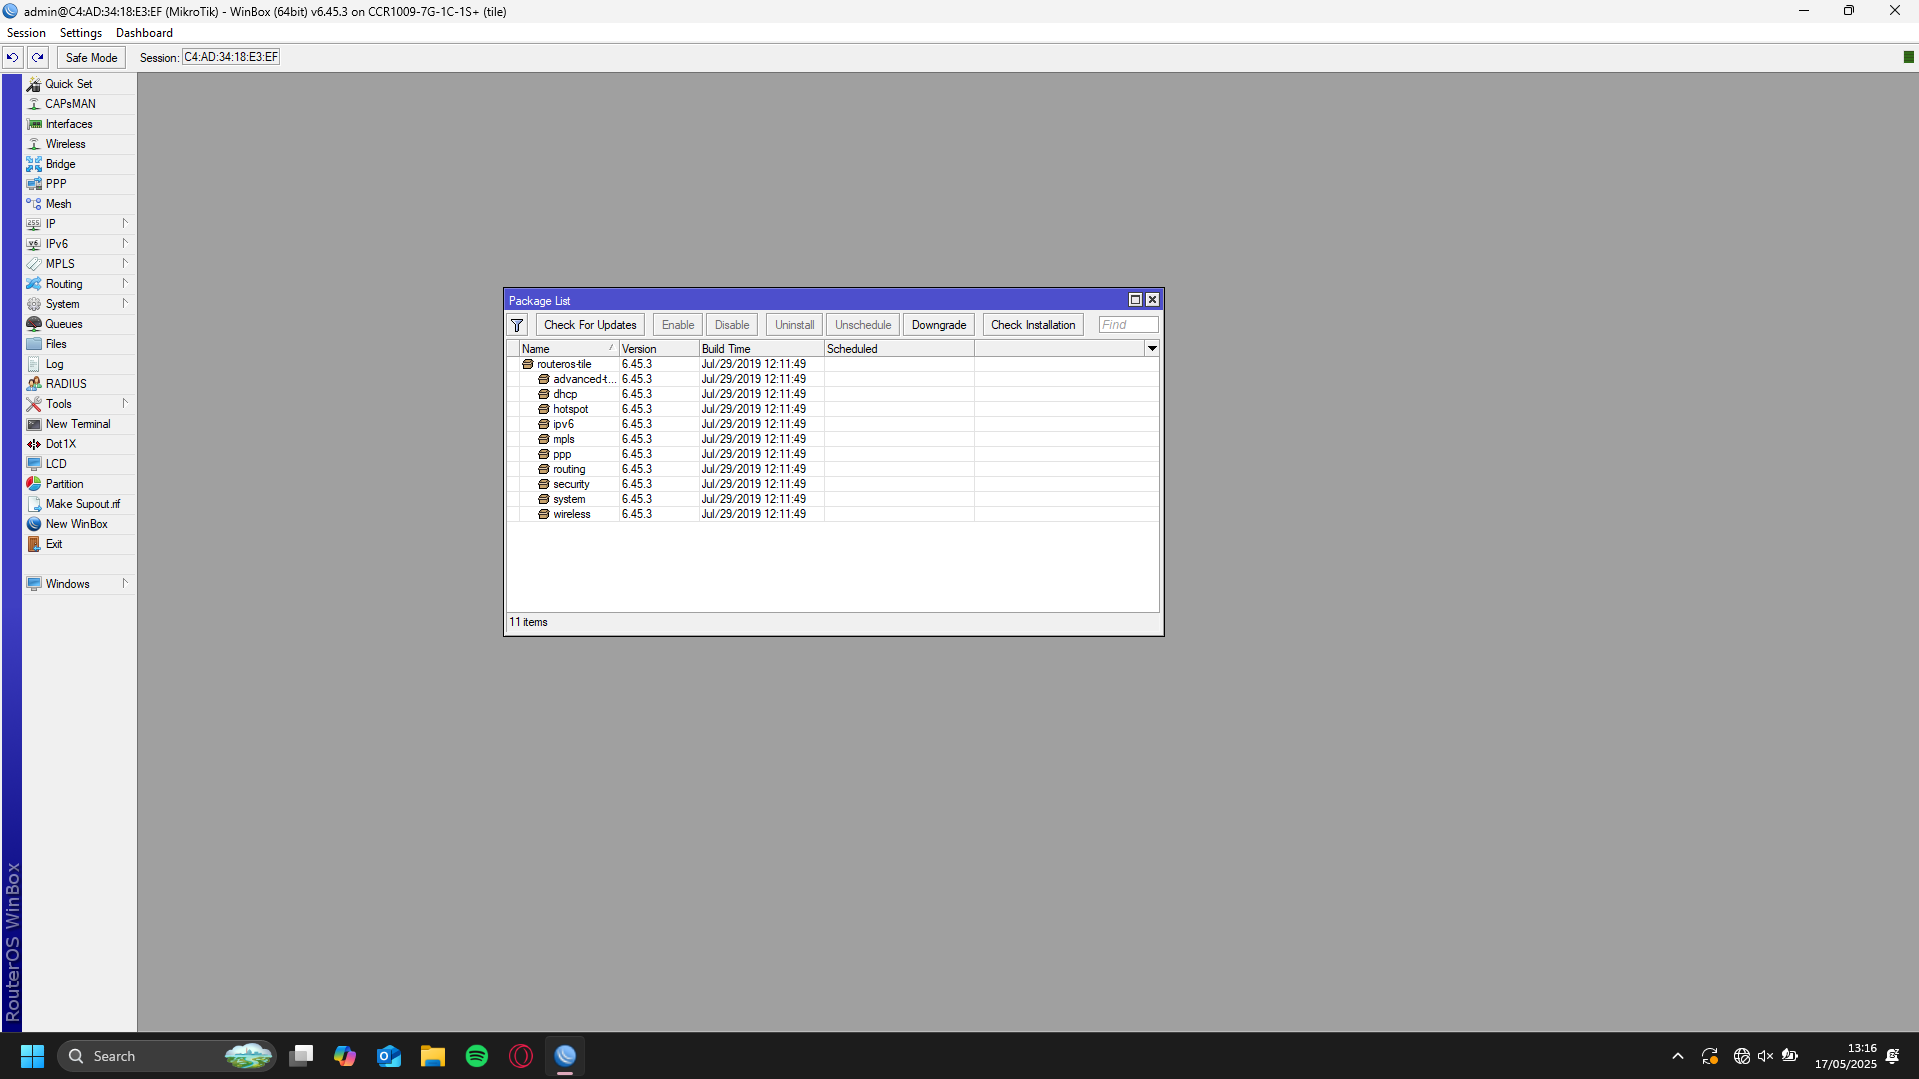
\includegraphics[width=0.48\textwidth]{P1/img/Package IPv6 PC1.png}
    \caption{Package IPv6 dari PC-1}
    \label{fig:crimping2_lampiran}
\end{figure}
\hfill

\newpage

\begin{figure}[H]
    \centering
    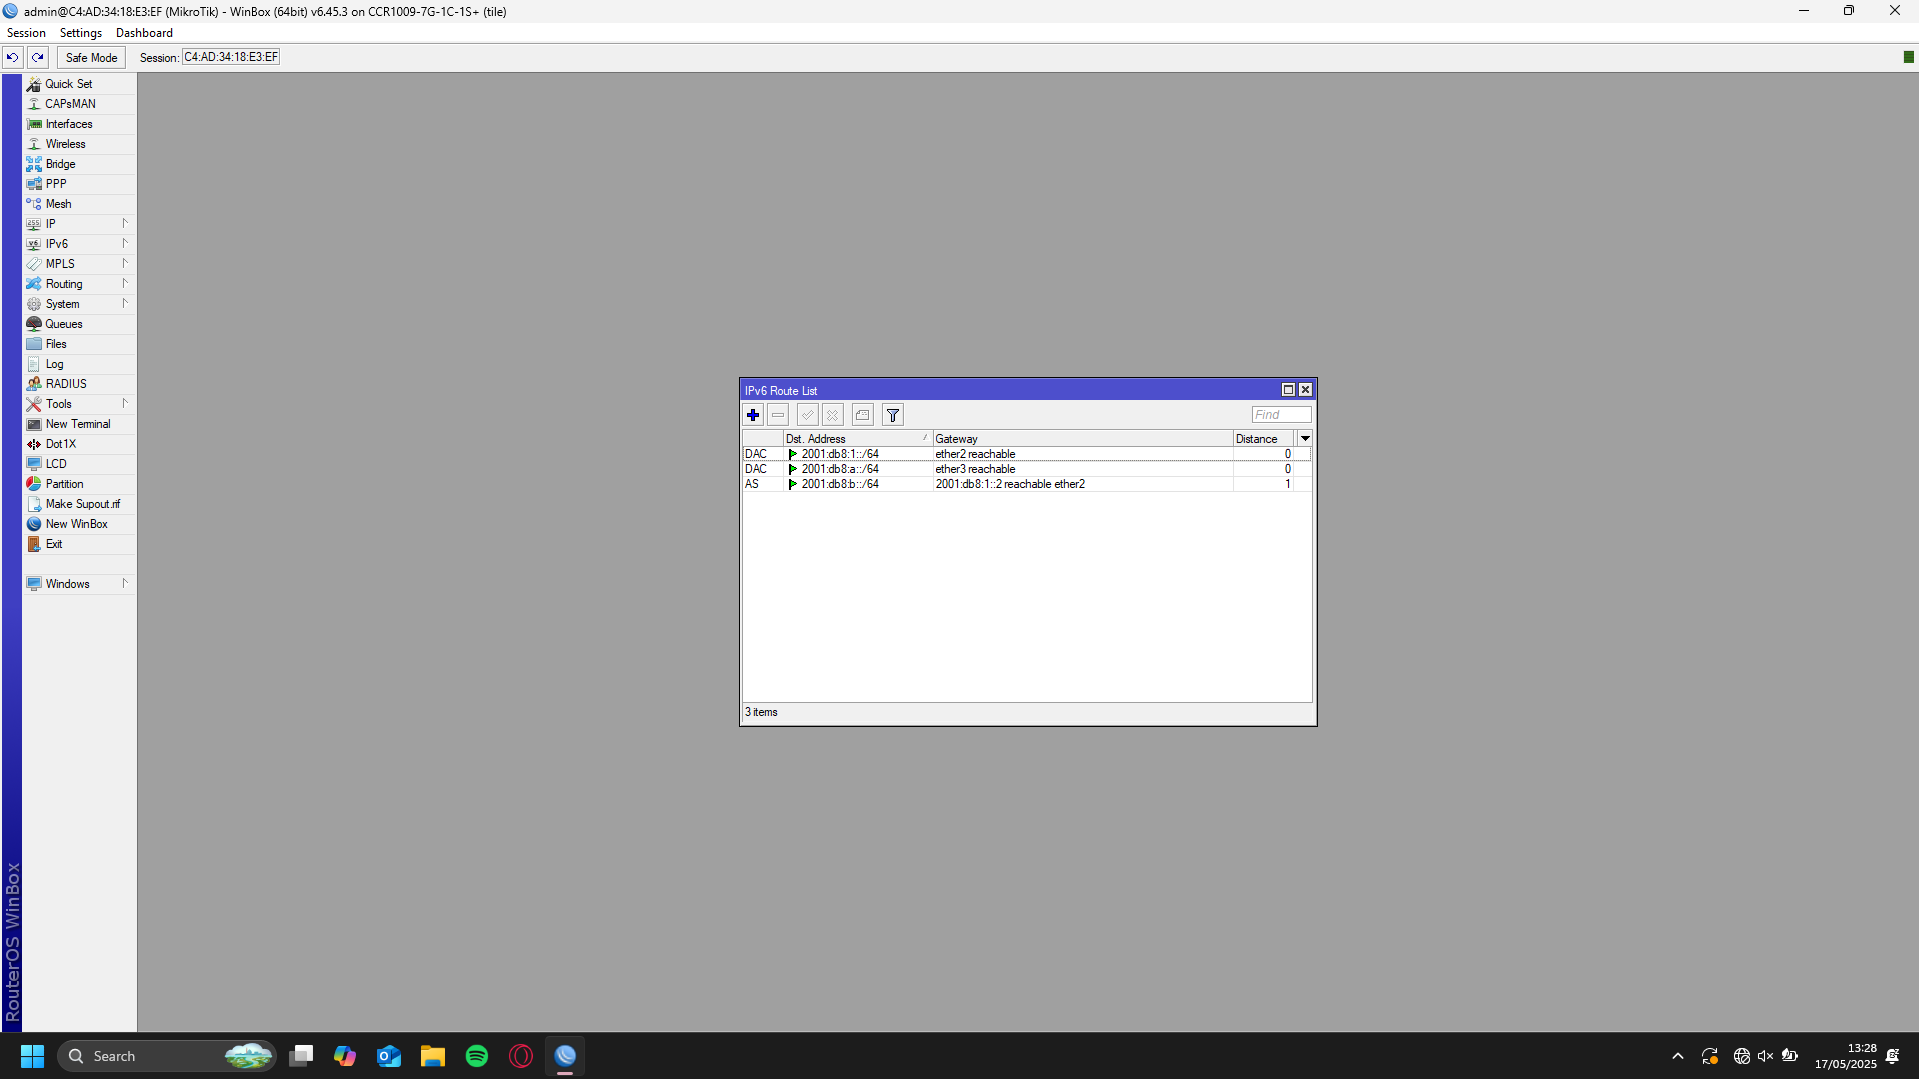
\includegraphics[width=0.48\textwidth]{P1/img/Route List PC1.png}
    \caption{Route List IPv6 dari PC-1}
    \label{fig:crimping2_lampiran}
\end{figure}
\hfill

\begin{figure}[H]
    \centering
    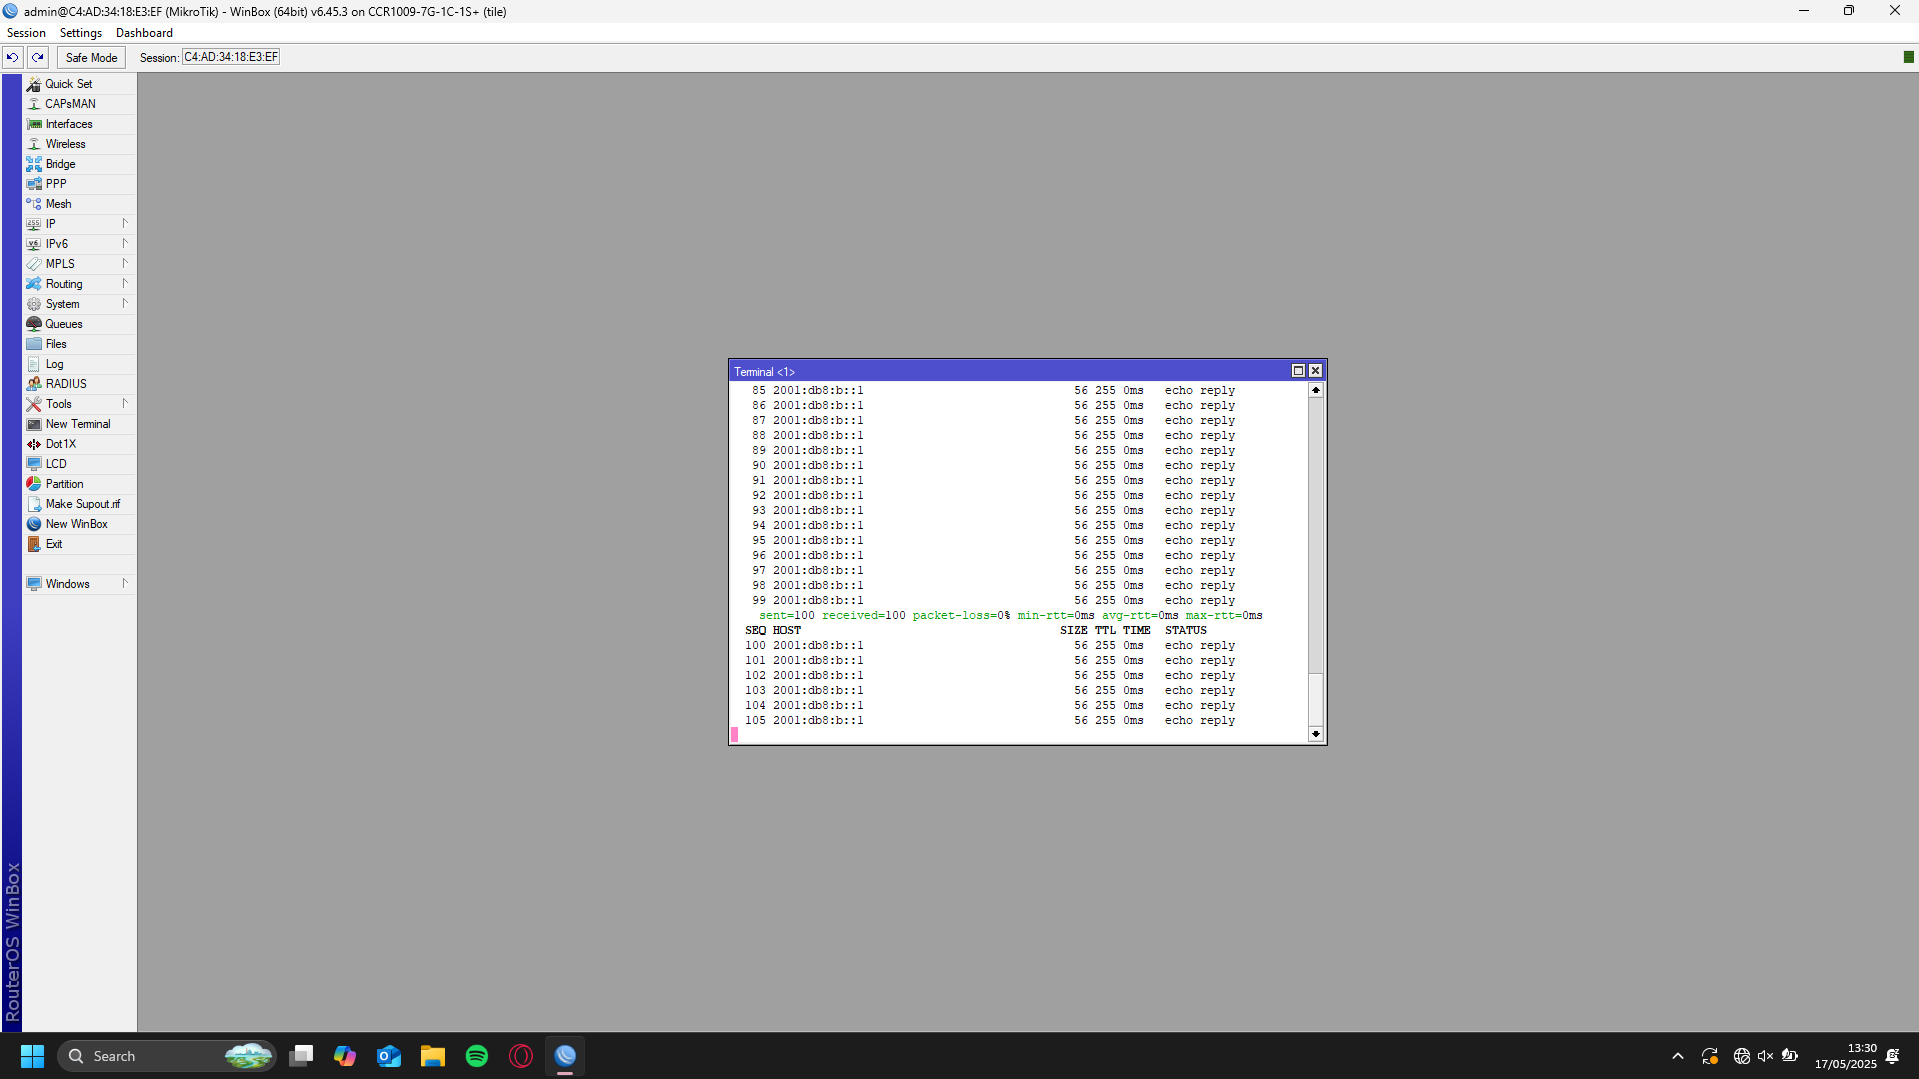
\includegraphics[width=0.48\textwidth]{P1/img/Hasil Ping Router1 ke Router2.png}
    \caption{Hasil Ping Routing Statis Antar Router}
    \label{fig:crimping2_lampiran}
\end{figure}
\hfill

\begin{figure}[H]
    \centering
    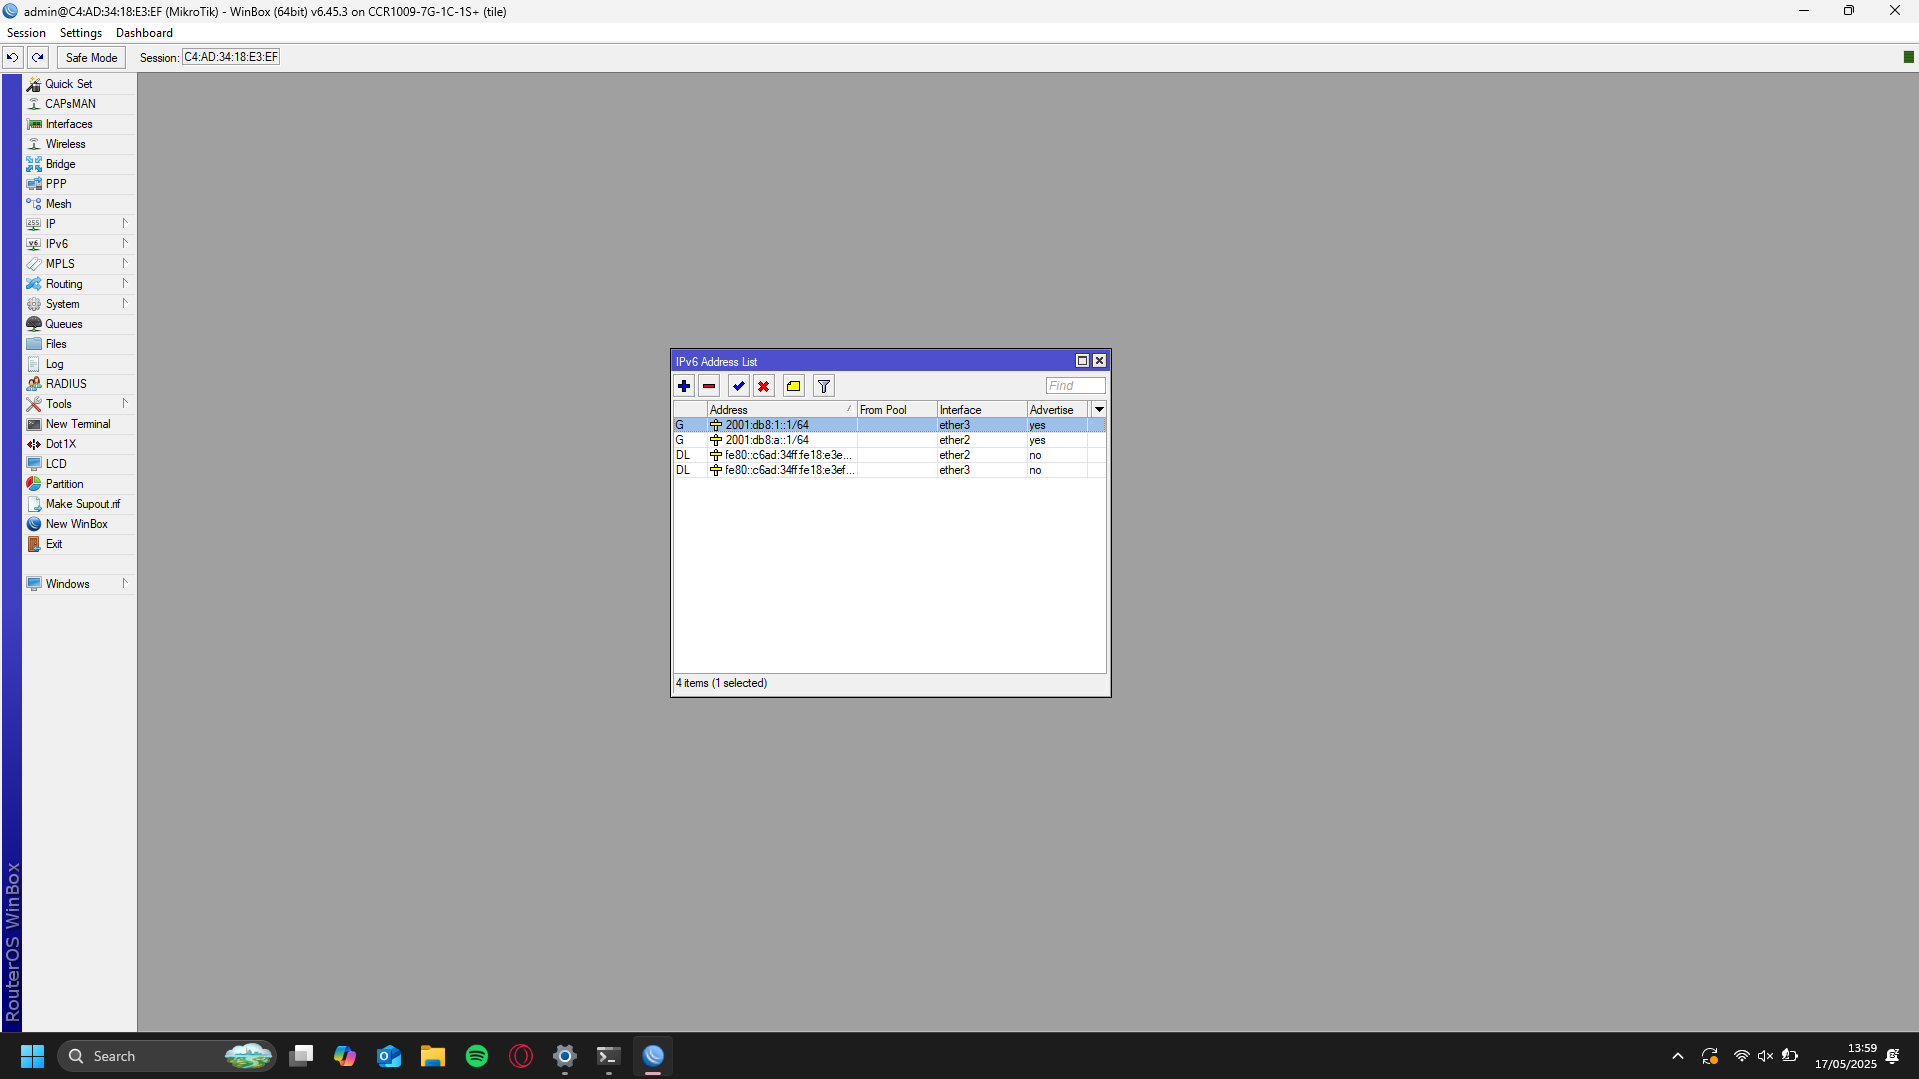
\includegraphics[width=0.48\textwidth]{P1/img/Address List IP Dinamis.png}
    \caption{Address List IP Routing Dinamis}
    \label{fig:crimping2_lampiran}
\end{figure}

\begin{figure}[H]
    \centering
    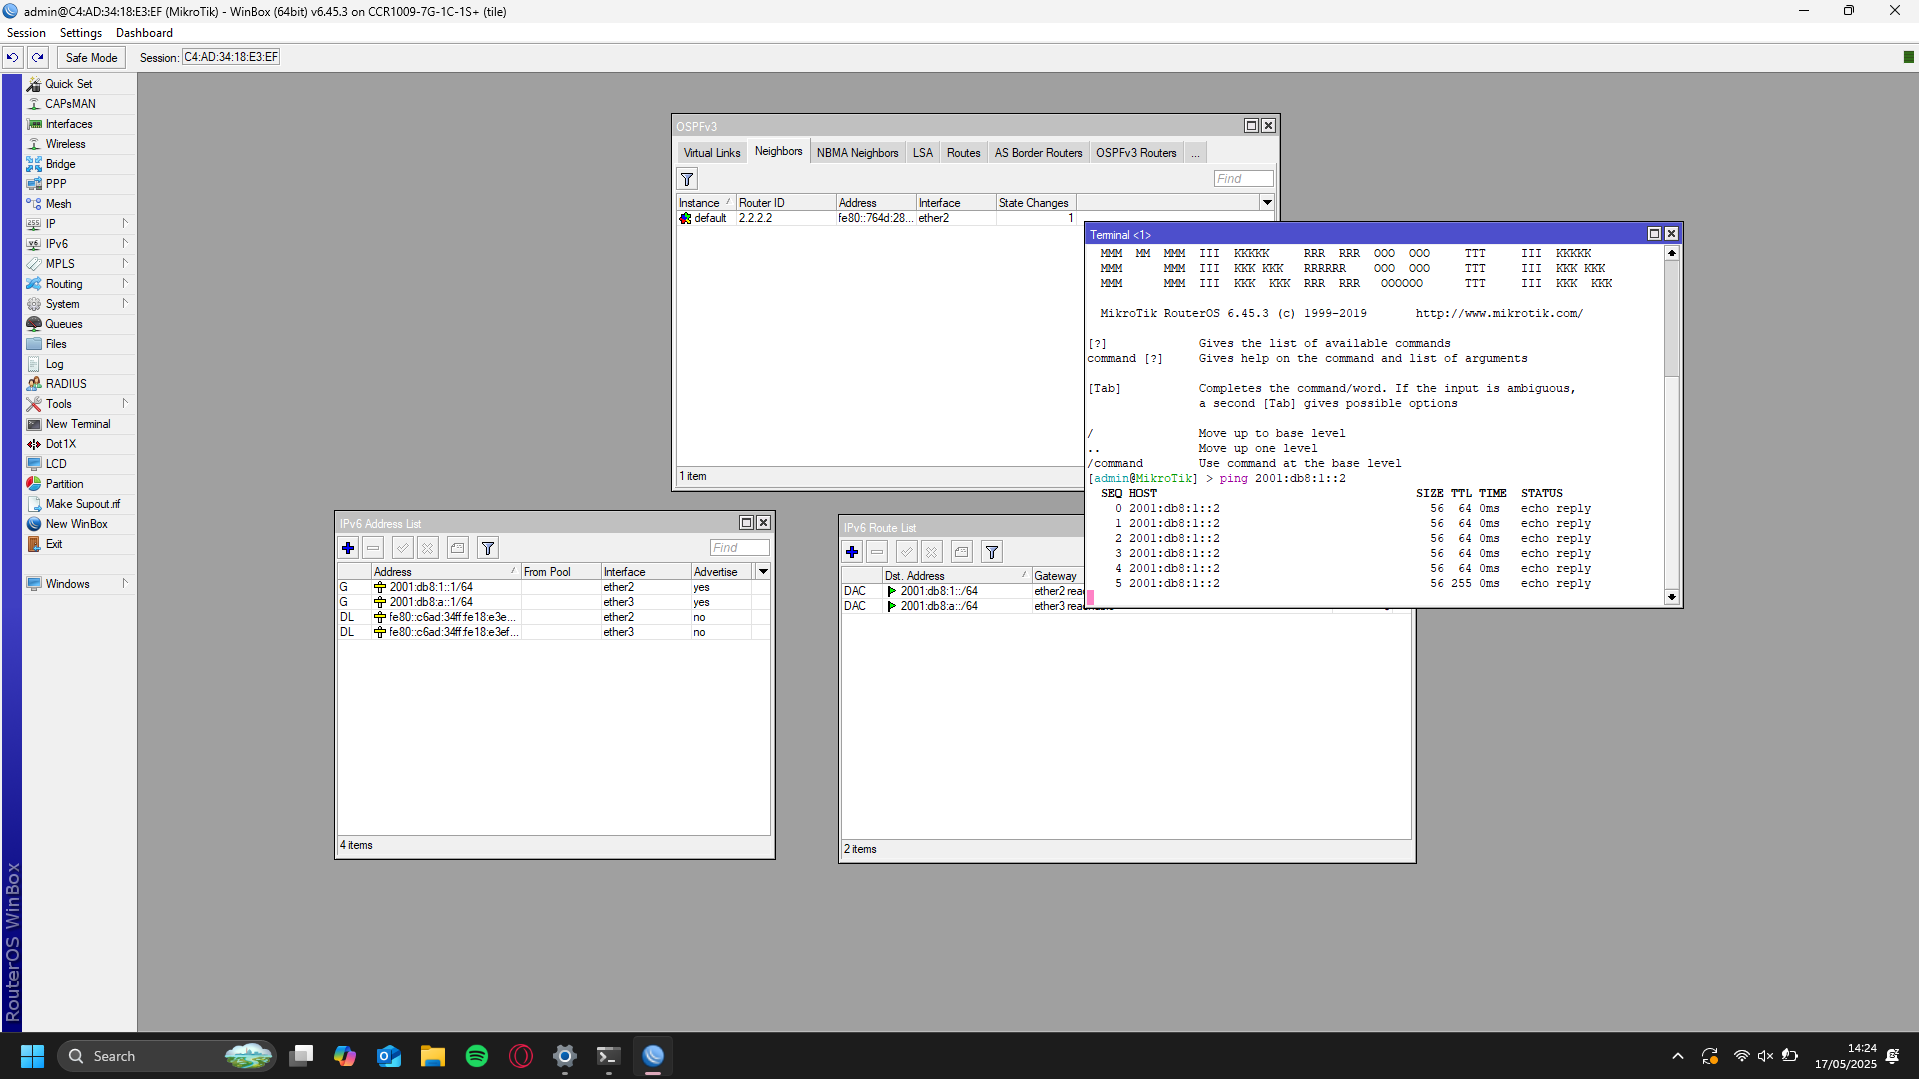
\includegraphics[width=0.48\textwidth]{P1/img/Hasil Ping Dinamis Router1 ke Router2.png}
    \caption{Hasil Ping Routing Dinamis Antar Router}
    \label{fig:crimping2_lampiran}
\end{figure}

\begin{figure}[H]
    \centering
    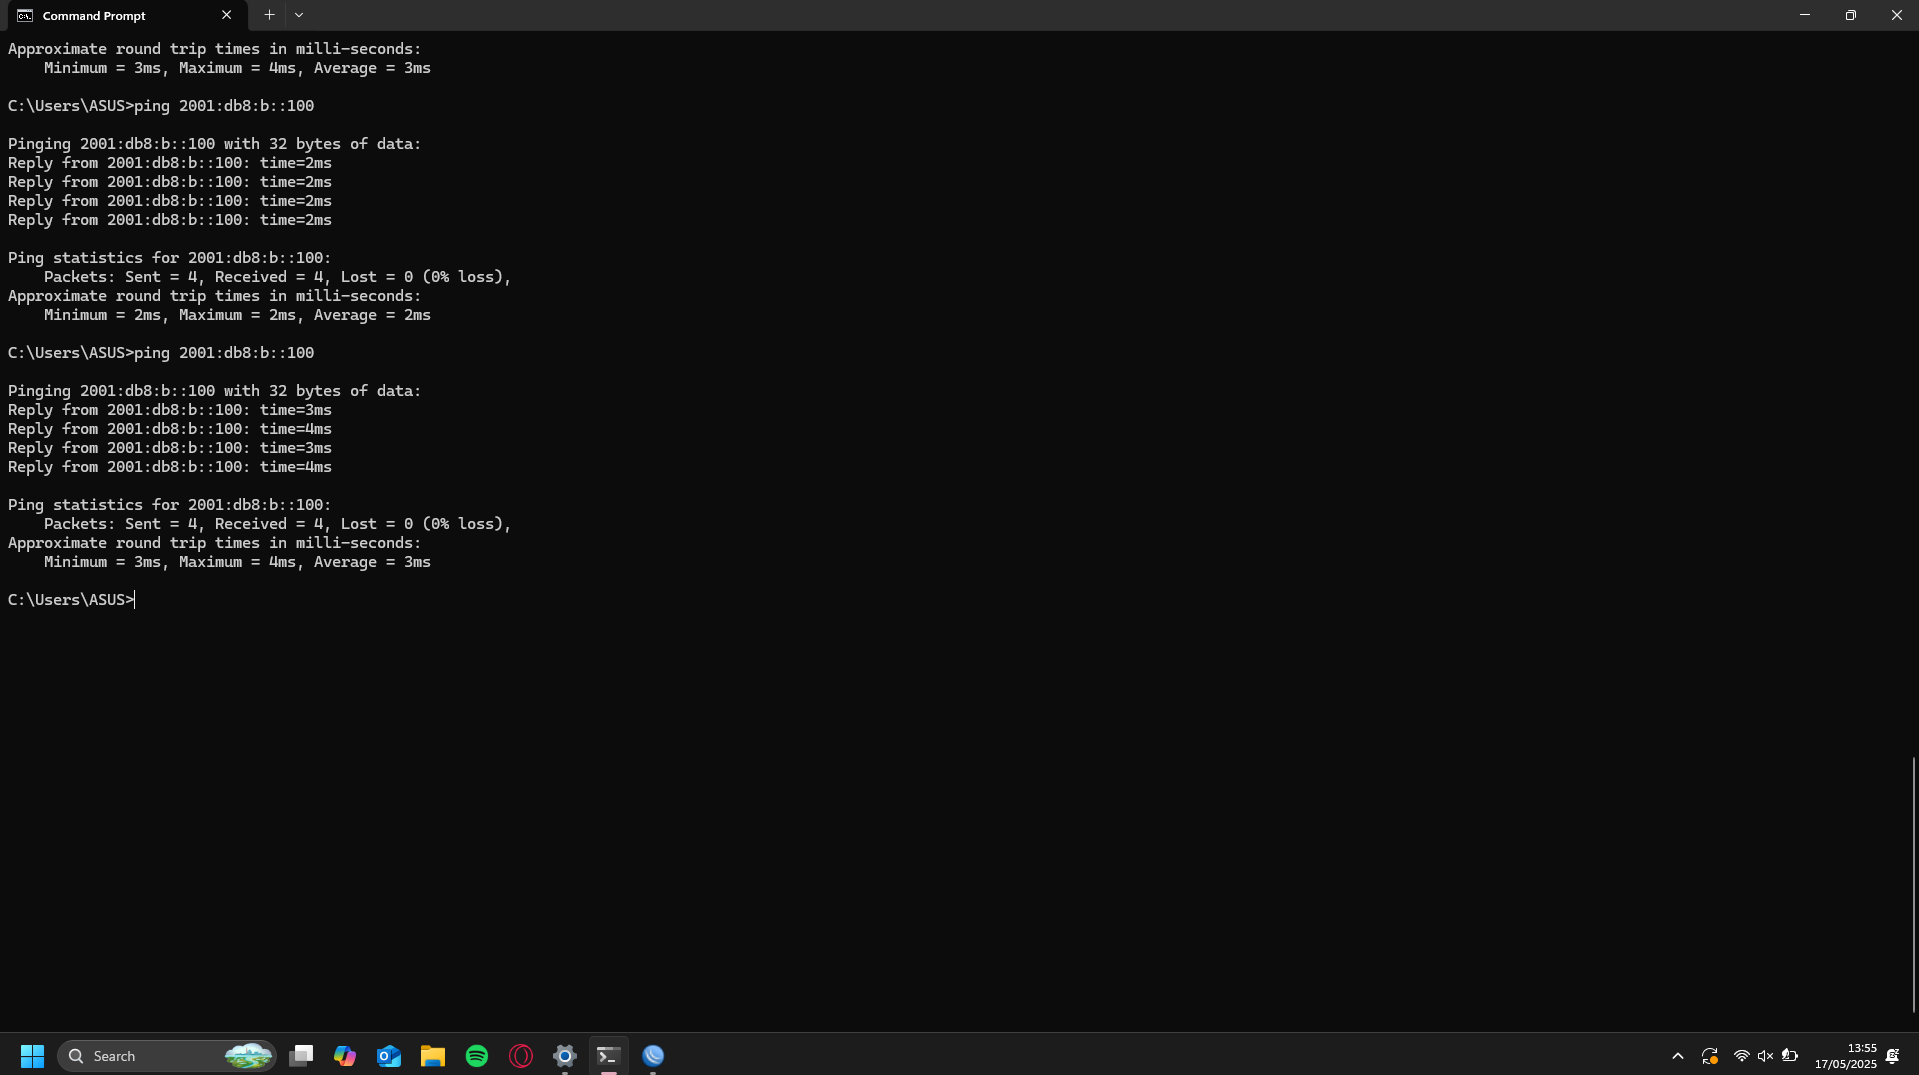
\includegraphics[width=0.48\textwidth]{P1/img/Hasil Ping PC1 ke PC2.png}
    \caption{Hasil Ping Antar PC}
    \label{fig:crimping2_lampiran}
\end{figure}


